\chapter{Uso de la librería}
	
	Este capítulo se presenta como resultado del presente trabajo. Dada la extensión de la librería, no resulta posible ni deseable mostrar el código fuente completo\footnote{El código completo puede ser consultado y descargado desde la página \url{https://github.com/HugoRedon/Materia}. El apéndice \ref{chap:github} guía al lector en el procedimiento de modificación o extensión del código fuente.} en este documento, en cambio se mostrarán pequeños fragmentos de código mostrando la forma de utilizar la librería y su estructura.
		\section{Ecuación de estado cúbica}
 La presión es el cálculo mas sencillo que podemos realizar con la ecuación de estado cúbica.

\begin{equation}
	p = \frac{R T}{v-b} - \frac{a}{v^2 +u b v + w b^2 }
\end{equation}

 Crearemos una clase en java que use la librería Materia y realize una gráfica de presión contra volumen a una temperatura determinada.

%\pgfplotstabletypeset{plotdata/pressurevolume.dat}%no es necesario mostrar la tabla

\begin{tikzpicture}
\begin{axis}
\addplot[blue]table{plotdata/pressurevolume.dat};
\end{axis}
\end{tikzpicture}


\begin{tikzpicture}
\begin{axis}
\addplot3[surf,
colormap={blueblack}{color=(white) color=(blue)},
domain=0:1]table{plotdata/pressurevolumetemperature.dat};
\end{axis}
\end{tikzpicture}


\begin{lstlisting}[label=se,caption=Some Code]
Cubic cubic = new Cubic();
//parametros de van der waals para el heptano
double a = 3107000.0;
double b = 0.2049;


double min_volume = 0.245;
double max_volume = 2.06;

int n = 100;
double pass = (max_volume- min_volume)/n;

PrintWriter writer = new PrintWriter(fileName, "UTF-8");
writer.println(" Volumen Presion");
for(int i=0;i < n; i++){
	double volume = min_volume + pass*i;
	double pressure = cubic.calculatePressure(300, volume, a, b);
	
	writer.println(" "+ volume + " " + pressure);
}
writer.close();		
\end{lstlisting}
















%hecho
		\subsection{Factor de compresibilidad}\label{subsec:compresibilityFactor}

Es necesario realizar la solución de la ecuación de estado cúbica para conocer el factor de compresibilidad. La solución de la ecuación se realiza en el método ``calculateCompresibilityFactor'' de la clase ``Cubic''.

El método recibe los parámetros adimensionales A, B y la fase a la cual se desea calcular el factor de compresibilidad. La clase ``Cubic'' tiene los métodos necesarios para transformar los parámetros a y b a su forma adimensional A y B.

El el fragmento de código \ref{lst:compresibility} se muestra la creación de la ecuación de estado cúbica, adimensionalización de los parámetros y finalmente el cálculo de el factor de compresibilidad.

\begin{lstlisting}[label=lst:compresibility,caption={Cálculo del factor de compresibilidad, y adimensionamiento de los parámetros a y b con la clase ``Cubic''}]
Cubic cubic = EquationsOfState.vanDerWaals();
		
double criticalTemperature = 540.2;
double criticalPressure = 2.74000E+06;

double pressure = criticalPressure * 1.5;
double reducedTemperature= criticalTemperature * 2;

//parametros de van Der Waals para el heptano
double a = 3107000.0;
double b = 0.2049;

double A =cubic.get_A(temperature, pressure, a);
double B = cubic.get_B(temperature, pressure, b);

double z =cubic.calculateCompresibilityFactor(A, B, Phase.LIQUID);
\end{lstlisting}
 
	Gracias a esta librería podemos formar los diagramas de la figura \ref{fig:zchart}.

\begin{figure}
\begin{tabular}{c c}
	\begin{tikzpicture}
	\begin{axis}[width=0.45\linewidth,font=\footnotesize,view/v=-6,
		ylabel= {Presión reducida },
		xlabel= {Temperatura reducida},
		zlabel={Factor de compresibilidad z}]%[colormap/hot]
	\addplot3[surf,point meta=explicit] table[meta=rt,x=p,y=rt,z=z]{plotdata/compresibilitiChart/pz_temp.dat};
	\end{axis}
	\end{tikzpicture}
	&
	\begin{tikzpicture}
	\begin{axis}[width=0.45\linewidth,font=\footnotesize,
		xlabel= {Presión reducida },
		ylabel= {Factor de compresibilidad z}]%[colormap/hot]
	\addplot[blue]table{plotdata/compresibilitiChart/pz_temp.dat};
	\end{axis}
	\end{tikzpicture}
\end{tabular}
\caption{Diagramas del factor de compresibilidad }
\label{fig:zchart}
\end{figure}
%hecho
		\subsection{Parámetros de la ecuación de estado cúbica}

\begin{equation}
	b_i = \Omega_b \frac{R T_{ci}}{p_{ci}} 
\end{equation}

\begin{equation}
 a_i = \Omega_a \frac{\left(R T_{ci}\right)^2}{p_{ci}} \alpha_i
\end{equation}

En las secciones anteriores se usaron los parámetros a y b de la eq. de estado cúbica para el heptano. 

Estos parámetros dependen de la eq. de estado cúbica, expresión de \alpha y si la ecuación es utilizada para representar a una mezcla también dependen de la regla de mezclado.

La expresión de $\alpha$ puede ser una función de la temperatura





\begin{figure}[!h]
  
  \centering
    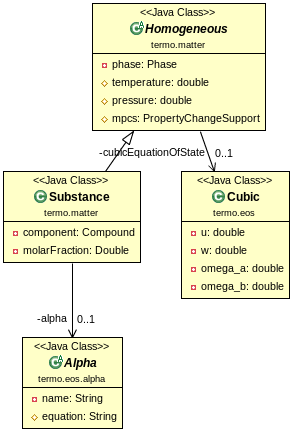
\includegraphics[scale=0.7]{cubic.png}
    \caption{A picture of a gull.}
\end{figure}




		\subsection{Entalpía}

\begin{equation}
h = h^{\neq} + \left[ \frac{T(\frac{\partial a}{\partial T}) - a}{b\sqrt{u²-4w} }\right] 
\ln\left[\frac{2v+b\left(u + \sqrt{u²-4w}\right)}{2v+b\left(u - \sqrt{u²-4w}\right)}\right]
+ pv - RT
\end{equation}

\begin{lstlisting}[label=some-code,caption=Some Code]
private  double calculateEnthalpy( double volume){
    double idealGasEnthalpy = calculateIdealGasEnthalpy();
    double a = calculate_a_cubicParameter();
    double b = calculate_b_cubicParameter();
    double L = cubicEquationOfState.calculateL(volume, b);
    double partial_aPartial_temperature = partial_aPartial_temperature( );
    
    return idealGasEnthalpy + ((partial_aPartial_temperature - a)/b) * L  + pressure * volume - Constants.R *temperature;
}
\end{lstlisting}	


\subsubsection{Entalpía del gas ideal}
\begin{equation}
h^{\neq} = \sum_{i=1}^{nc} x_i \left[ h_i^{ref} + \int_{Tref}^{T} Cp_i^{\neq} \mathrm{d}T \right]
\end{equation}



\begin{tikzpicture}
\begin{axis}
\addplot[blue]table{plotdata/enthalpy/lv.dat};
\end{axis}
\end{tikzpicture}


%\addplot+[point meta=explicit]table[x=xcolname,y=ycolname,meta=colordata]{datafile.dat};%ejemplo de uso meta
\begin{tikzpicture}
\begin{axis}[view/h=-165]
\addplot3[surf,point meta=explicit]table[meta=temperature]{plotdata/enthalpy/lv3d.dat};
\addplot3[surf,point meta=explicit]table[meta=temperature]{plotdata/enthalpy/l3d.dat};
\addplot3[surf,point meta=explicit]table[meta=temperature]{plotdata/enthalpy/v3d.dat};
\end{axis}
\end{tikzpicture}
\begin{tikzpicture}
\begin{axis}[view/h=-225]
\addplot3[surf]table{plotdata/enthalpy/lv3d.dat};
\addplot3[surf]table{plotdata/enthalpy/l3d.dat};
\addplot3[surf]table{plotdata/enthalpy/v3d.dat};
\end{axis}
\end{tikzpicture}
\begin{tikzpicture}
\begin{axis}[view/h=-120]
\addplot3[surf]table{plotdata/enthalpy/lv3d.dat};
\addplot3[surf]table{plotdata/enthalpy/l3d.dat};
\addplot3[surf]table{plotdata/enthalpy/v3d.dat};
\end{axis}
\end{tikzpicture}	

		
		\subsection{Expresiones de $\alpha$}

	\subsubsection{Soave\cite{soave}}

\begin{gather}
	\alpha^{\nicefrac{1}{2}} = 1 + m \left(1-\sqrt{T_r}\right)\\
	m = 0.48508+1.55171\omega-0.15613\omega^2
\end{gather}
	\subsubsection{Peng and Robinson \cite{pengRobinson}}


\begin{gather}
	\alpha^{\nicefrac{1}{2}} = 1 + m \left(1-\sqrt{T_r}\right)\\
	m = 0.37464+1.54226\omega-0.2699\omega^2
\end{gather}
	\subsubsection{Mathias\cite{mathias} }
\begin{itemize}

\item{$T < T_C$}
\begin{gather}
	\alpha^{\nicefrac{1}{2}} = 1 + m \left(1-\sqrt{T_r}\right)- A\left(1-T_r\right)\left(0.7-T_r\right)
	\\
	m = 0.48508+1.55191\omega-0.15613\omega^2
\end{gather}

\item{$T > T_c$}
\begin{gather}
	\alpha = \exp{\left[ \left( \frac{c-1}{c} \right)  \left(  1- T_r^c  \right)  \right]}\\
	c = 1 + \frac{m}{2} + 0.3 A
\end{gather}

 \end{itemize}


	\subsubsection{Stryjek and Vera(PRSV)\cite{stryjekVeraPureCompounds} }
\begin{itemize}

\item{$T < T_C$}
\begin{gather}
	\alpha^{\nicefrac{1}{2}} = 1 + \kappa_0 \left(1-\sqrt{T_r}\right)- \kappa_1\left(1-T_r\right)\left(0.7-T_r\right)
	\\
	\kappa_0 = 0.378893+1.4897153\omega-0.17131848\omega^2+0.0196554\omega³
\end{gather}

\item{$T > T_c$}
\begin{equation}
	\alpha^{\nicefrac{1}{2}} = 1 + \kappa_0\left(1- \sqrt{T_r}\right)
\end{equation}

 \end{itemize}	
	\subsubsection{Adachi and Lu \cite{adachiLu}}

\begin{equation}
\alpha = A\cdot {10}^{B\left(1-T_r\right)}
\end{equation}
	\subsubsection{Soave \cite{soaveR}}

\begin{equation}
\alpha= 1+\left(1-T_r\right)\left(A + \frac{B}{T_r}\right)
\end{equation}
	\subsubsection{Melhem, et al.\cite{melhem}}

\begin{equation}
\ln{\alpha}=A\left(1-T_r\right)+ B\left(1-\sqrt{T_r}\right)^2
\end{equation}
	\subsubsection{Androulakis,et al.\cite{androulakis}}

\begin{itemize}
\item{$T < T_C$}
\begin{equation}
 \alpha = 1 + A \left(1-T_r^{\nicefrac{2}{3}}\right) + B\left(1-T_r^{\nicefrac{2}{3}}\right)^2+ C\left(1-T_r^{\nicefrac{2}{3}}\right)^3
\end{equation}
\item{$T > T_c$}
\begin{equation}
\alpha = \mathrm{e}^{A\left(1-T_r^{\nicefrac{2}{3}}\right)}
\end{equation}
\end{itemize}
	\subsubsection{Mathias and Copeman. \cite{mathiasCopeman,michelsen}}

\begin{itemize}
\item{$T < T_c$}
\begin{equation}
\alpha^{\nicefrac{1}{2}} = 1 + A\left(1-\sqrt{T_r}\right) + B\left(1-\sqrt{T_r}\right)^2 + C\left(1-\sqrt{T_r}\right)^3
\end{equation}
\item{$T > T_c$}
\begin{equation}
\alpha^{\nicefrac{1}{2}} = 1 + A\left(1-\sqrt{T_r}\right)\footnote{La ecuación no se incluyó en el trabajo original de Mathias and Copeman\cite{mathiasCopeman}; esta expresión fue incorporada en el trabajo de Dahl and Michelsen \cite{michelsen}}
\end{equation}
\end{itemize}
	\subsubsection{Yu and Lu\cite{yuLu}}

\begin{itemize}
\item{$T < T_c$}
\begin{equation}
 \log_{10}{\alpha} = \left(A+B T_r+ C T_r^2\right)\left(1-T_r\right)
\end{equation}
\item{$T > T_c$}
\begin{equation}
 \log_{10}{\alpha} = \left(A+B+C \right)\left(1-T_r\right)
\end{equation}
\end{itemize}
	\subsubsection{Stryjek and Vera\cite{stryjekVera}}

\begin{itemize}
\item{$T < T_c$}
\begin{gather}
\alpha^{\nicefrac{1}{2}} = 1 + \kappa\left(1-\sqrt{T_r}\right)\\
\kappa = m + \left[
		A+ B\left(C- T_r\right)\left(1-\sqrt{T_r}\right)
	\right]
	\left[
		\left(1+ \sqrt{T_r}\right)\left(0.7-T_r\right)
	\right]\\
m=0.378893 + 1.4897153 \omega - 0.17131848 \omega^2+ 0.0196554 \omega^3
\end{gather}
\item{$T > T_c$}
\begin{equation}
\alpha^{\nicefrac{1}{2}} = 1 + m\left(1-\sqrt{T_r}\right)
\end{equation}
\end{itemize}
	\subsubsection{Twu\cite{twuequation}}
\begin{equation}
	\alpha = T_r^{N\left(M-1\right)}\exp{\left(L\left(1-T_r^{N M}\right)\right)}
\end{equation}
	\subsubsection{Twu \cite{twuactivity}}
\begin{itemize}
\item{$T < T_c$}
\begin{gather}
\alpha = \alpha^{(0)} + \omega\left(\alpha^{(1)}-\alpha^{(0)}\right)\\
\text{Para}\qquad \alpha^{(0)}\notag\\
L= 0.196545\qquad M=0.906437\qquad N=1.26251\\
\text{Para}\qquad \alpha^{(1)}\notag\\
L=0.704001 \qquad M =0.790407 \qquad N=2.13076
\end{gather}
\item{$T > T_c$}
\begin{gather}
\alpha = \alpha^{(0)} + \omega\left(\alpha^{(1)}-\alpha^{(0)}\right)\\
\text{Para}\qquad \alpha^{(0)}\notag\\
L= 0.358826\qquad M=4.23478\qquad N=-0.2\\
\text{Para}\qquad \alpha^{(1)}\notag\\
L=0.0206444 \qquad M =1.22942 \qquad N=-8.0
\end{gather}
\end{itemize}
	\subsubsection{GCEOS (AspenHYSYS)}

\begin{gather}
\alpha^{\nicefrac{1}{2}} = 1 + \kappa \left(1 - \sqrt{T_r}\right)\\
\kappa = \kappa_0 + \left[ 
	\kappa_1 + \left(   \kappa_2 - \kappa_3 T_r   \right)
	\left(1 - T_r^{\kappa_4}\right) 
\right]
\left[
	\left(1 + \sqrt{T_r}\right)\left(0.7 - T_r\right)
\right]
T^{\kappa_5}\\
\kappa_0 = A + B \omega+ C \omega^2+ D \omega^3
\end{gather}









		
		\subsection{Fugacidad}

\begin{multline}
\ln\hat{\phi_i} = - \ln\left(\frac{v-b}{v}\right) 
+ (z-1)\left[\frac{1}{b}\frac{\partial bN}{\partial N_i}\right]
+ \frac{a}{RTb\sqrt{u^2-4w}}
\\
\left[\frac{1}{b}\frac{\partial bN}{\partial N_i}
- \frac{1}{aN}\frac{\partial aN²}{\partial N_i}\right]
\ln\left[\frac{2v+b\left(u + \sqrt{u²-4w}\right)}{2v+b\left(u - \sqrt{u²-4w}\right)}\right]
-\ln{z}
\end{multline}
		
		\subsection{Entropía}
\begin{equation}
s = s^{\neq} + R\ln\left[\frac{z(v-b)}{v}\right] + \frac{\frac{\partial a}{\partial T}}{b \sqrt{u^2 - 4w}}
\ln\left[\frac{2v+b\left(u + \sqrt{u²-4w}\right)}{2v+b\left(u - \sqrt{u²-4w}\right)}\right]
\end{equation}
\begin{equation}
s^{\neq} = \sum_{i=1}^{nc} x_i\left[s_i^{ref} + \int_{Tref}^T \frac{Cp_i^{\neq}}{T} \mathrm{d}T 
- R\ln \left(\frac{p}{p_{ref}}\right)- R\ln{x_i}
\right]
\end{equation}
		\subsection{Energía libre de Gibbs}

\begin{equation}
g = h - T * s;
\end{equation}
		
		\subsection{volumen molar}
		\subsection{Equilibrio LV}
			\subsubsection{Temperatura de Burbuja}



\begin{tikzpicture}[nodes={draw, fill=white,align=center},row sep=0.3cm,column sep=0.5cm] ]

\node(init){Inicio};
\node[below of=init] (lab)  {Lectura de \textbf{Datos} \\$P,x_1, x_2,\ldots, x_{nc}$};
\node[below of=lab,below](estim){Estimado inicial de\\ las incognitas\\$T,y_1,y_2,\ldots,y_{nc}$};
\node[below of=estim,below](relations){Cálculo de las\\ razones de equilibrio\\
$K_i = \frac{ \hat{\phi}_i^L }{\hat{ \phi}_i^V}$};
\node[below of=relations,below = 0.2cm](error){Cálculo de la función Error\\$ S_y =\sum_{i=1}^{nc} K_i x_i $\\$ E = \ln{S_y} $};

\node[below of=error,below](criteria){$|E| \leq 1\cdot10^{-4}\quad \text{o} \quad  1\cdot 10^{-5}$};
\node[below of=criteria,below](tempIncrement){Incrementer la temperatura\\$T^* = T + \Delta T$\\
$\Delta T = 0.1  \quad \text{o} \quad 1.0 K$};

\node[below of=tempIncrement,below](relationsWithIncrement){Cálculo de las Razones\\ de Equilibrio con $T^*$
\\$K_i^* = \frac{ \hat{\phi}_i^L }{ \hat{\phi}_i^V}$};

\node[right of=criteria	,right=2.2cm](end){Fin};


\node[right of=tempIncrement, right=3cm](errorWithIncrement){Cálculo de la función Error \\ con $T^*$\\
$ S_y^* =\sum_{i=1}^{nc} K_i^* x_i $\\$ E^* = \ln{S_y^*} $};

\node[right of=relations, right = 3cm](newValues){Cálculo de las nuevas estimaciones \\ de las \textbf{Incógnitas}\\
\begin{minipage}{0.2\linewidth}
\begin{equation*}
T_{nueva} = \frac{TT^* \left(E^*-E\right)}{T^*E^*-TE}
\end{equation*}
\begin{equation*}
 S_y =\sum_{i=1}^{nc} K_i x_i \\
 \end{equation*}
 \begin{equation*}
\left(y_i\right)_{nueva} = \frac{K_i x_i}{S_y}
\end{equation*}
\end{minipage}
};


\draw[-latex] (init)--(lab);
\draw[-latex] (lab)--(estim);
\draw[-latex] (estim)--(relations);
\draw[-latex] (relations)--(error);
\draw[-latex] (error)--(criteria);
\draw[-latex] (criteria)--node[fill=none,draw=none,above]{SI}(end);
\draw[-latex] (criteria)--node[fill=none,draw=none,left]{NO}(tempIncrement);
\draw[-latex] (tempIncrement)--(relationsWithIncrement);
\draw[-latex] (relationsWithIncrement)--(errorWithIncrement);
\draw[-latex] (errorWithIncrement)--(newValues);
\draw[-latex] (newValues)--(relations);

\end{tikzpicture}

		\subsubsection{Temperatura de Rocío}



\begin{tikzpicture}[nodes={draw, fill=white,align=center},row sep=0.3cm,column sep=0.5cm] ]

\node(init){Inicio};
\node[below of=init] (lab)  {Lectura de \textbf{Datos} \\$P,y_1, y_2,\ldots, y_{nc}$};
\node[below of=lab,below](estim){Estimado inicial de\\ las incognitas\\$T,x_1,x_2,\ldots,x_{nc}$};
\node[below of=estim,below](relations){Cálculo de las\\ razones de equilibrio\\
$K_i = \frac{ \hat{\phi}_i^L }{ \hat{ \phi}_i^V}$};
\node[below of=relations,below = 0.2cm](error){Cálculo de la función Error\\
$ S_x =\sum_{i=1}^{nc}\frac{y_i}{ K_i} $\\$ E = \ln{S_x} $};

\node[below of=error,below](criteria){$|E| \leq 1\cdot10^{-4}\quad \text{o} \quad  1\cdot 10^{-5}$};
\node[below of=criteria,below](tempIncrement){Incrementer la temperatura\\$T^* = T + \Delta T$\\
$\Delta T = 0.1  \quad \text{o} \quad 1.0 K$};

\node[below of=tempIncrement,below](relationsWithIncrement){Cálculo de las Razones\\ de Equilibrio con $T^*$\\$K_i^* = \frac{ \hat{\phi}_i^L }{\hat{\phi}_i^V}$};

\node[right of=criteria	,right=2.2cm](end){Fin};


\node[right of=tempIncrement, right=3cm](errorWithIncrement){Cálculo de la función Error \\ con $T^*$\\
$ S_x^* =\sum_{i=1}^{nc} \frac{y_i}{K_i^*}  $\\$ E^* = \ln{S_x^*} $};

\node[right of=relations, right = 3cm](newValues){Cálculo de las nuevas estimaciones \\ de las \textbf{Incógnitas}\\
\begin{minipage}{0.2\linewidth}
\begin{equation*}
T_{nueva} = \frac{TT^* \left(E^*-E\right)}{T^*E^*-TE}
\end{equation*}
\begin{equation*}
 S_x =\sum_{i=1}^{nc}\frac{y_i}{K_i}   \\
 \end{equation*}
 \begin{equation*}
\left(x_i\right)_{nueva} = \frac{y_i}{K_i S_x}
\end{equation*}
\end{minipage}
};


\draw[-latex] (init)--(lab);
\draw[-latex] (lab)--(estim);
\draw[-latex] (estim)--(relations);
\draw[-latex] (relations)--(error);
\draw[-latex] (error)--(criteria);
\draw[-latex] (criteria)--node[fill=none,draw=none,above]{SI}(end);
\draw[-latex] (criteria)--node[fill=none,draw=none,left]{NO}(tempIncrement);
\draw[-latex] (tempIncrement)--(relationsWithIncrement);
\draw[-latex] (relationsWithIncrement)--(errorWithIncrement);
\draw[-latex] (errorWithIncrement)--(newValues);
\draw[-latex] (newValues)--(relations);

\end{tikzpicture}

		\subsubsection{Presión de Burbuja}




\begin{tikzpicture}[nodes={draw, fill=white,align=center},row sep=0.3cm,column sep=0.5cm] ]

\node(init){Inicio};
\node[below of=init] (lab)  {Lectura de \textbf{Datos} \\$T,x_1, x_2,\ldots, x_{nc}$};
\node[below of=lab,below](estim){Estimado inicial de\\ las incognitas\\$P,y_1,y_2,\ldots,y_{nc}$};
\node[below of=estim,below](relations){Cálculo de las\\ razones de equilibrio\\
$K_i = \frac{ \hat{\phi}_i^L }{\hat{ \phi}_i^V}$};
\node[below of=relations,below = 0.2cm](error){Cálculo de la función Error\\$ S_y =\sum_{i=1}^{nc} K_i x_i $\\$ E = {S_y}-1 $};

\node[below of=error,below](criteria){$|E| \leq 1\cdot10^{-4}\quad \text{o} \quad  1\cdot 10^{-5}$};
\node[below of=criteria,below](pressureIncrement){Incrementer la temperatura\\$P^* = P + \Delta P$\\
$\Delta P = 0.001  \quad \text{o} \quad 0.0001 K$};

\node[below of=pressureIncrement,below](relationsWithIncrement){Cálculo de las Razones\\ de Equilibrio con $P^*$
\\$K_i^* = \frac{ \hat{\phi}_i^L }{ \hat{\phi}_i^V}$};

\node[right of=criteria	,right=2.2cm](end){Fin};


\node[right of=pressureIncrement, right=3cm](errorWithIncrement){Cálculo de la función Error \\ con $P^*$\\
$ S_y^* =\sum_{i=1}^{nc} K_i^* x_i $\\$ E^* = S_y^* -1 $};

\node[right of=relations, right = 3cm](newValues){Cálculo de las nuevas estimaciones \\ de las \textbf{Incógnitas}\\
\begin{minipage}{0.2\linewidth}
\begin{equation*}
T_{nueva} = \frac{P P^* \left(E^*-E\right)}{P^*E^*-P E}
\end{equation*}
\begin{equation*}
 S_y =\sum_{i=1}^{nc} K_i x_i \\
 \end{equation*}
 \begin{equation*}
\left(y_i\right)_{nueva} = \frac{K_i x_i}{S_y}
\end{equation*}
\end{minipage}
};


\draw[-latex] (init)--(lab);
\draw[-latex] (lab)--(estim);
\draw[-latex] (estim)--(relations);
\draw[-latex] (relations)--(error);
\draw[-latex] (error)--(criteria);
\draw[-latex] (criteria)--node[fill=none,draw=none,above]{SI}(end);
\draw[-latex] (criteria)--node[fill=none,draw=none,left]{NO}(pressureIncrement);
\draw[-latex] (pressureIncrement)--(relationsWithIncrement);
\draw[-latex] (relationsWithIncrement)--(errorWithIncrement);
\draw[-latex] (errorWithIncrement)--(newValues);
\draw[-latex] (newValues)--(relations);

\end{tikzpicture}

		\subsubsection{Presión de Rocío}



\begin{tikzpicture}[nodes={draw, fill=white,align=center},row sep=0.3cm,column sep=0.5cm] ]

\node(init){Inicio};
\node[below of=init] (lab)  {Lectura de \textbf{Datos} \\$T,y_1, y_2,\ldots, y_{nc}$};
\node[below of=lab,below](estim){Estimado inicial de\\ las incognitas\\$P,x_1,x_2,\ldots,x_{nc}$};
\node[below of=estim,below](relations){Cálculo de las\\ razones de equilibrio\\
$K_i = \frac{ \hat{\phi}_i^L }{ \hat{ \phi}_i^V}$};
\node[below of=relations,below = 0.2cm](error){Cálculo de la función Error\\
$ S_x =\sum_{i=1}^{nc}\frac{y_i}{ K_i} $\\$ E = S_x-1 $};

\node[below of=error,below](criteria){$|E| \leq 1\cdot10^{-4}\quad \text{o} \quad  1\cdot 10^{-5}$};
\node[below of=criteria,below](tempIncrement){Incrementer la temperatura\\$P^* = P + \Delta P$\\
$\Delta P = 0.001  \quad \text{o} \quad 0.0001 K$};

\node[below of=tempIncrement,below](relationsWithIncrement){Cálculo de las Razones\\ de Equilibrio con $P^*$\\$K_i^* = \frac{ \hat{\phi}_i^L }{\hat{\phi}_i^V}$};

\node[right of=criteria	,right=2.2cm](end){Fin};


\node[right of=tempIncrement, right=3cm](errorWithIncrement){Cálculo de la función Error \\ con $P^*$\\
$ S_x^* =\sum_{i=1}^{nc} \frac{y_i}{K_i^*}  $\\$ E^* = S_x^*-1 $};

\node[right of=relations, right = 3cm](newValues){Cálculo de las nuevas estimaciones \\ de las \textbf{Incógnitas}\\
\begin{minipage}{0.2\linewidth}
\begin{equation*}
T_{nueva} =P- \frac{E  \left(P^*-P\right)}{E^*-E}
\end{equation*}
\begin{equation*}
 S_x =\sum_{i=1}^{nc}\frac{y_i}{K_i}   \\
 \end{equation*}
 \begin{equation*}
\left(x_i\right)_{nueva} = \frac{y_i}{K_i S_x}
\end{equation*}
\end{minipage}
};


\draw[-latex] (init)--(lab);
\draw[-latex] (lab)--(estim);
\draw[-latex] (estim)--(relations);
\draw[-latex] (relations)--(error);
\draw[-latex] (error)--(criteria);
\draw[-latex] (criteria)--node[fill=none,draw=none,above]{SI}(end);
\draw[-latex] (criteria)--node[fill=none,draw=none,left]{NO}(tempIncrement);
\draw[-latex] (tempIncrement)--(relationsWithIncrement);
\draw[-latex] (relationsWithIncrement)--(errorWithIncrement);
\draw[-latex] (errorWithIncrement)--(newValues);
\draw[-latex] (newValues)--(relations);

\end{tikzpicture}

		\subsection{Flash}



\begin{tikzpicture}[nodes={draw, fill=white,align=center},row sep=0.3cm,column sep=0.5cm] ]

\node(init){Inicio};
\node[below of=init] (lab)  {Lectura de \textbf{Datos} \\$T,P,z_1, z_2,\ldots, z_{nc}$};
\node[below of=lab,below](estim){Estimado inicial de\\ las incognitas\\$V/F,x_1,x_2,\ldots,x_{nc}$\\$y_1,y_2 \ldots, y_{nc}$};
\node[below of=estim,below](relations){Cálculo de las\\ razones de equilibrio\\
$K_i = \frac{ \hat{\phi}_i^L }{ \hat{ \phi}_i^V}$};
\node[below of=relations,below = 0.2cm](error){Cálculo de la función Error\\
$ \zeta =\sum_{i=1}^{nc}\left| x_i \hat{\varphi}_i^L - y_i \hat{\varphi}_i^V \right|$};

\node[below of=error,below](criteria){$|\zeta| \leq 1\cdot10^{-4}\quad \text{o} \quad  1\cdot 10^{-5}$};


\node[below of=criteria,below](rachford){Cálculo de $V/F$ con Rachford-Rice:\\ 
\begin{minipage}{0.5\linewidth}
\begin{equation*}
S = \sum_{i=1}^{nc}\frac{z_i\left(K_i - 1\right)}{1+ \frac{V}{F}\left(K_i-1\right)}
\end{equation*}
Encontrar $V/F$ tal que $S = 0$\\
Método de Newton-Raphson\\
\begin{equation*}
\acute{S} = \sum_{i=1}^{nc} \frac{-z_i \left(K_i - 1\right)^2}{\left[1+ \frac{V}{F} \left(K_i-1\right)\right]^2}
\end{equation*}
\begin{equation*}
\left(\frac{V}{F}\right)_{nueva} = \left(\frac{V}{F}\right) - \frac{S}{\acute{S}}
\end{equation*}
\end{minipage}};

\node[right of=criteria	,right=2.2cm](end){Fin};


\node[right of=estim, right = 3cm](newValues){Cálculo de las nuevas estimaciones \\ de las \textbf{Incógnitas}\\
\begin{minipage}{0.3\linewidth}
\begin{equation*}
\acute{x_i} = \frac{z_i}{1 + \frac{V}{F}\left(K_i-1\right)}
\end{equation*}
\begin{equation*}
 S_x =\sum_{i=1}^{nc}\acute{x}_i \qquad x_i = \frac{\acute{x_i}}{S_x}
\end{equation*}
\begin{equation*}
\acute{y_i} = \acute{x_i} K_i = \frac{z_i K_i}{1+\frac{V}{F}\left(K_i - 1\right)}
\end{equation*}
\begin{equation*}
 S_y =\sum_{i=1}^{nc}\acute{y}_i \qquad y_i = \frac{\acute{y_i}}{S_y}
\end{equation*}
\end{minipage}
};


\draw[-latex] (init)--(lab);
\draw[-latex] (lab)--(estim);
\draw[-latex] (estim)--(relations);
\draw[-latex] (relations)--(error);
\draw[-latex] (error)--(criteria);
\draw[-latex] (criteria)--node[fill=none,draw=none,above]{SI}(end);
\draw[-latex] (criteria)--node[fill=none,draw=none,left]{NO}(rachford);

\draw[-latex] (rachford)-|(newValues);
\draw[-latex] (newValues)--(relations);

\end{tikzpicture}

		\subsection{Diagramas}
	
